\documentclass[conference, letterpaper, 10pt]{IEEEtran}

\usepackage[utf8]{inputenc}

\title{On the security of encryption and compression composition under reflection attacks}

%\author{
%    Anonymized submission
%}

 \author{
     \IEEEauthorblockN{Dimitris Karakostas}
     \IEEEauthorblockA{University of Athens \\
     dimit.karakostas@gmail.com}
     \and
     \IEEEauthorblockN{Aggelos Kiayias}
     \IEEEauthorblockA{University of Edinburgh\\
     akiayias@inf.ed.ac.uk}
     \and
     \IEEEauthorblockA{Dionysis Zindros}
     \IEEEauthorblockA{University of Athens \\
     dionyziz@di.uoa.gr}
 }

\usepackage{url}
\usepackage{amsmath}
\usepackage{graphicx}
\usepackage{listings}
\usepackage{mathtools}
\usepackage{amsfonts}
% \usepackage{amsthm}
\usepackage{amssymb}
\usepackage[colorlinks=true,linkcolor=blue,citecolor=green]{hyperref}

\usepackage{cite}

\DeclarePairedDelimiter{\ceil}{\lceil}{\rceil}
\let\oldemptyset\emptyset
\let\emptyset\varnothing

\newtheorem{lemma}{Lemma}

\newcommand\defeq{\stackrel{\mathclap{\normalfont\mbox{def}}}{=}}
\newcommand{\overbar}[1]{\mkern 1.5mu\overline{\mkern-1.5mu#1\mkern-1.5mu}\mkern 1.5mu}

\begin{document}

\maketitle

\begin{abstract}
When compression is composed with encryption, unexpected vulnerabilities can
arise. Such vulnerabilities have been explored in practical attacks against TLS
such as CRIME, TIME, and BREACH, even after TLS 1.3. We introduce an abstract
theoretical cryptographic model for such attacks, the \textit{adaptive
reflection security} game with the relevant security definitions. We propose a
model for \textit{compression idealness} and experimentally show that typical compression
functions expose partially ideal behavior. We then experimentally show that
typical plaintexts used in practice follow an interdependent joint distribution,
our stronger notion of dependent joint distributions. Based on these two
properties, we prove that \textit{compression-detectability} of predicates
arises, the ability to extract a predicate of the plaintext using reflection.
We then prove that all length-preserving encryption schemes are insecure when
composed with such functions. Our attack model describes two modes of attack,
one-shot and amplified. For the case of the BREACH attack, we discuss how it can
be described as an instance of our theoretical model. Motivated by the lack of
production-grade testing tools, we provide a modular scalable open-source
generic attack framework that implements compression side-channel attacks in a
robust manner. Finally, we propose a novel defense protocol, \textit{context
hiding}, that effectively eliminates the threat these attacks pose. This
protocol modifies the plaintext joint distribution so as to remove the
interdependence, thereby mitigating the problem. We show that our method of
defense performs significantly more favourably in terms of compression rate when
compared to previous techniques.
\end{abstract}

\section{Introduction}\label{sec:prev}

Compression and encryption composition has caused serious security problems
in protocols such as TLS \cite{c15} over the years. These
include attacks like CRIME \cite{c1}, TIME \cite{c2}, and BREACH \cite{c3}.

However, the theoretical models for these classes of attacks has been limited.
The compression side-channel attack was first studied by Kelsey \cite{c4} in 2002.
Kelley and Tamassia\cite{c5}  discuss the notion of \textit{entropy-restricted} semantic
security, but this only models the case where two secrets compress to the same
length, and so it is difficult to capture practical techniques used in attacks
such as BREACH.

Alawatugoda etc. \cite{c6} introduce a model for \textit{Cookie recovery},
\textit{Random cookie indistinguishability}, as well as \textit{Chosen cookie indistinguishability}.
Nevertheless, their security models are limited in classes of rendering functions
that are very specific. In their models, the attacker is able to directly influence
the output of the rendering function through concatenation. While their results
have significant value in analyzing the security of compression, we believe
a generalization and abstraction of the rendering process is essential to
theoretically analyzing the security of generic compression and rendering functions.
Furthermore, generalized rendering and compression functions help better
capture and model specific attacks such as BREACH in the context of
realistic instances, like the rendering of real web pages.

\subsection{A motivational example}\label{subsec:example}
Our work is highly motivated by the threat compression side-channel attacks pose
against real-world systems. The severity of these attacks can be highlighted by
the example that this section describes.

Consider the communication between a user that browses the Internet and a server
that hosts a website. This website might be a social network, e-banking service,
mail provider etc. When the server receives a request for a web page on the
website it collects all needed data, generates the HTML code that will be
displayed by the user's browser and sends a network response containing this
code along with other resources such as images, libraries etc. All response data
is encrypted using TLS which ensures privacy and integrity between the two
communicating parties.

Next we assume an adversary that aims at breaking this communication's security.
This adversary tries to decrypt multiple bits of encrypted information between
the user and the website and reveal information about the private data
exchanged. However, the adversary should fulfill the requirements described
below.

Firstly, he should be able to issue any number of malicious requests using the
user's cookies. This can be achieved by forcing the user's browser to run a
piece of code, such as a Javascript script hosted on an adversary-controlled
website, that requests some web page on said website.

Secondly, the requests should include an adversary-chosen string that is also
included in the response data. In order to achieve that, the website must offer
some web page that provides a HTTP GET parameter whose value is included in the HTML
response.

Finally, the adversary is able to handle all user's network traffic. That way he
is able to collect and analyze the network packets of the encrypted
communication with the server. He is also able inject the malicious script in
plain HTTP responses the user receives from third websites even when the user is
careful enough to avoid adversary-controlled websites.

The described adversary can issue a compression side-channel attack against the
user and the website. The malicious requests contain specially crafted
reflection strings that are included in the response and compressed with the
private data. The structure of the reflection depends heavily on properties of
the private data and will be further explored in the following sections.

As the attack progresses the adversary collects network data for multiple
requests and reflections. Although this data is encrypted, analysis on the
lengths of different request packets may reveal properties of the private data,
at which point the privacy of the communication between the user and the website is
broken.

A formal description of the above example is defined in Appendix \ref{sec:breachmodel}.

\subsection{Terms}
The previous example allows us to explore multiple terms that are used in the
rest of our work. These terms include the \textit{rendering function} $f$,
\textit{rendered message}, \textit{secret} $s$, \textit{noise} $v$,
\textit{reflection} $r$ and the distributions $\mathcal{M}$ and $\mathcal{V}$.

In order to elaborate on the previous example, we define a specific instance of
it. In this case, the website is found in the URL \textit{mail.example.com} and
the web page that the adversary exploits is
\textit{mail.example.com/search?query=attack}. This website provides a HTTP GET
parameter called \textit{query} and the adversary uses the reflection string
\textit{attack}. The HTML response is described below:

\begin{lstlisting}[basicstyle=\small]
<div>
    <p>You searched for: attack</p>
    <p>No results found.</p>
</div>
<div>
    Your inbox:
    <ul>
    <li>[Bank] Routing number: 123</li>
    </ul>
</div>
<div>
    <p>A random token: L*fKLs#a4fd@</p>
</div>
\end{lstlisting}

The server's HTML generator could be abstracted as a \textit{rendering
function} $f$. This function's input is the user's request, resources such as the
HTML blueprint for the web page, and external functions such as web framework
middlewares.

The output of the rendering function is the \textit{rendered message} $m$. This
is the generated HTML response code, that contains response data that is
rendered by the user's browser and contains different string elements. The HTML
response elements can be distinguished based on the role of each one in a
compression-based attack. An element can be a \textit{secret}, \textit{noise},
\textit{static}, or a \textit{reflection}. An element's alphabet consists of all
possible values each character in the element may take.

A \textit{secret} $s$ is any part of the response that is user-specific and a
potential security risk in case of compromise. Examples of secrets in an HTML
response include private messages, email contents, financial data, or web
security elements like CSRF tokens \cite{c16}. The secret's alphabet is generally printable
text characters. In our example, the strings "Bank", which refers to a email
topic, and "Routing number: 123", which represents an email content, are
considered secrets.

The \textit{noise} $v$ on the other side is a value that changes unpredictably per
request regardless of the requested content. Examples of noise include
timestamps, user-generated content, masked information. The noise's distribution
is in general a random distribution of a subset of printable characters. In our
example, the string "L*fKLs!a4fd@" is considered noise.

\textit{Static} content is any part of the response that remains unchanged
across user requests like HTML $<$div$>$ tags and CSS code. Static content is fully
predictable per request and thus irrelevant in the attack outcome since the
attacker can bypass it. Strings like "div", "ul", "Your inbox:" are considered
static in our example.

A \textit{reflection} $r$ is a component crafted by the attacker and can be
adaptively transformed as the attack progresses. The reflection is included in
the response and compressed in the same context with the secret that is
targeted. In our example, the HTTP GET value "attack" of parameter "query" is used as
a reflection.

Secrets and reflections are chosen from the distribution $\mathcal{M}$. For
example, consider the secret "123" in our example. Two cases for the
distribution $\mathcal{M}$ would be all permutations of 4-length strings
consisting of printable characters or only english alphabet letters. The
reflection is chosen from the distribution $\mathcal{M}$, so the definition of
$\mathcal{M}$ reflects the adversary's power, i.e. in the first case above the
adversary is less powerful than the second.

Finally, a noise element is chosen from the distribution $\mathcal{V}$. This
distribution in our example describes the uniformly random choice of strings of
certain alphabet. In our example this alphabet is the printable ASCII characters
and a noise element is chosen randomly from $\mathcal{V}$ per request.

\subsection{Contributions}
Our contributions are two-fold. Firstly, we introduce a novel model for discussing
compression and encryption composition attacks, the \textit{adaptive reflection
game} with an accompanying security definition. This model is quite general in
that it does not describe specific instances of the rendering function $f$ or
the compression function $Com$. Furthermore, it allows for general distributions
of secret $\mathcal{M}$ and distributions of noise $\mathcal{V}$ which can
affect the rendering. Additionally, the model describes an adaptive attack,
but also allows for adaptive rendering based on the adversary behavior in the
general case. We then introduce the abstract property of \textit{compression detectability}
which we argue is a property commonly attained by compression functions when
composed with real-world rendering functions. Finally, we show that this somewhat
innocent property directly allows the construction of an attacker, which we
prove breaks the security of the scheme. We also prove that such
attacks can be amplified to achieve better confidence.

Secondly, we implement a production-grade general implementation of compression
and encryption composition attacks in the form of an open source framework and
tool which we call Rupture \cite{c7}. This generic framework provides an
extensible mechanism for experimentally testing attack and defense techniques
in a modular setting. We implement specific compression attack instances such
as BREACH. While limited proof-of-concept source code has been released for
compression side-channel attacks, as far as we know this is the first time
a working tool is provided for this class of attacks.

\section{Reflection security}\label{sec:refsec}

\subsection{Adaptive reflection game}\label{subsec:refsecgame}

Let $\mathcal{PE} = (\mathcal{K}, \mathcal{E}, \mathcal{D})$ be a public-key
encryption scheme, $\mathcal{A}$ be an adversary and $\mathcal{S}$ be a
simulator of $\mathcal{A}$.  The game
$\text{Game}_{\text{REF-SEC}}^{\mathcal{PE},\mathcal{A}}(\lambda,  f,
\mathcal{V}, g)$ is parameterized with a rendering function $f(\cdot, \cdot,
\cdot)$, a noise distribution $\mathcal{V}$, the security parameter $\lambda$,
some function $g$ of the plaintext vector, and a distribution of secrets $\mathcal{M}_\omega$
such that $\forall \omega \forall s \in \mathcal{M}_\omega: |s| = \lambda$. Notice
that the distribution of secrets is parameterized with the history of execution
$\omega$.

The challenger produces a $\lambda$-bit key $(pk, sk) \leftarrow
\mathcal{K}(\lambda)$. The adversary is given $pk$, $\mathcal{V}$, $g$ and $f$.
Setting $\omega = ()$, the empty vector, the challenger initially chooses
a secret $s_0 \leftarrow \mathcal{M}_\omega$.

The adversary is then allowed to run and make arbitrary calls to a reflection
oracle, which responds potentially differently to every round $i$. The oracle
is parameterized by $s_i$, the secret unknown to the
adversary.  For the reflection oracle call, the adversary chooses a reflection
string $r$ and sends it to the oracle. The oracle produces a noise string
$v \leftarrow \mathcal{V}$ and computes $m_i = f(s_i, r, v)$. Subsequently
$m_i$ is encrypted as $c_i = \mathcal{E}_\kappa(m_i)$, and $c_i$ is sent back
to the adversary. Once $m_i$ is computed, the history vector $\omega$ is updated
with the rendered message as $\omega = \omega : m_i$ where $:$ denotes appending
a vector element to an existing vector, and the next secret $s_{i+1} \leftarrow \mathcal{M}_\omega$
is chosen.

When the adversary decides to complete the game, they output a guess $y$. The
adversary is successful if $g(\psi) = y$, where $\psi$ is the sequence
of all secrets sampled by the reflection oracle during the course of the game.

Formally, let the public key adversarial game be defined as follows:

\begin{lstlisting}[texcl,mathescape,basicstyle=\small]
def $\text{Game}_{\text{REF-SEC}}^{\mathcal{PE},\mathcal{A}}(\lambda, f, \mathcal{V}, \mathcal{M}, g)$:
    $(pk, sk) \leftarrow \mathcal{K}(\lambda)$
    $\omega = ()$
    $i = 0$
    $y \leftarrow \mathcal{A}^{\text{Reflect}^{\mathcal{E}_{pk}, \mathcal{V}}}
     (\lambda, f, \mathcal{V}, \mathcal{M}, g)$
    if $y = g(\psi)$:
        return 1
    else:
        return 0
\end{lstlisting}

Where the reflection oracle provided to the adversary is as follows:

\begin{lstlisting}[texcl,mathescape,basicstyle=\small]
def $\text{Reflect}^{\mathcal{E}_{pk}, \mathcal{V}}(r)$: (global variable $\psi$)
    $s \leftarrow \mathcal{M}_\omega$
    $v \leftarrow \mathcal{V}$
    $m = f(s, r, v)$
    $\omega = \omega || m$
    $\psi = \psi || s$
    $c \leftarrow \mathcal{E}_{pk}(m)$
    return $c$
\end{lstlisting}

Let the simulator game be defined as follows:

\begin{lstlisting}[texcl,mathescape,basicstyle=\small]
def $\text{Game}_{\text{REF-SIM}}^{\mathcal{PE},\mathcal{S}}(\lambda, f, \mathcal{V}, \mathcal{M}, g)$:
    $\omega = ()$
    $i = 0$
    $y \leftarrow \mathcal{A}^{\text{ReflectSim}^{\mathcal{E}_{pk}, \mathcal{V}}}
     (\lambda, f, \mathcal{V}, \mathcal{M}, g)$
    if $y = g( \psi )$:
        return 1
    else:
        return 0
\end{lstlisting}

Where the simulator reflection oracle is configured to not answer:

\begin{lstlisting}[texcl,mathescape,basicstyle=\small]
def $\text{ReflectSim}^{\mathcal{E}_{pk}, \mathcal{V}}(r)$:
    $s \leftarrow \mathcal{M}_\omega$
    $v \leftarrow \mathcal{V}$
    $m = f(s, r, v)$
    $\omega = \omega || m$
    $\psi = \psi || s$
    return $\bot$
\end{lstlisting}

\subsection{Adversarial advantage}\label{subsec:refsecadv}

Let us now define the advantage of the adversary against a simulator:
\begin{align*}
    \text{Adv}_{\mathcal{PE}, \mathcal{A}, \mathcal{S}}&(\lambda, f, \mathcal{V}, \mathcal{M}, g) &\defeq\\
    |\Pr[\text{Game}_{\text{REF-SEC}}^{\mathcal{PE},\mathcal{A}}(\lambda, f, \mathcal{V}, \mathcal{M}, g) = 1] &-\\
    \Pr[\text{Game}_{\text{REF-SIM}}^{\mathcal{PE},\mathcal{S}}(\lambda, f, \mathcal{V}, \mathcal{M}, g) = 1]| &
\end{align*}

\subsection{Adaptive reflection security}\label{subsec:adaptiverefsec}

Given a polynomially computable rendering function $f(\cdot, \cdot, \cdot)$ and
a  noise distribution $\mathcal{V}$, a public-key encryption scheme
$\mathcal{PE}$ is \textit{reflection-secure} if:
\begin{align*}
\forall \mathcal{M}:
\forall g:
\forall PPT \mathcal{A}:
\exists PPT \mathcal{S}:\\
\text{Adv}_{\mathcal{PE}, \mathcal{A}, \mathcal{S}}(\lambda, f, \mathcal{V}, \mathcal{M}, g) = negl(\lambda)
\end{align*}

\subsection{Non-adaptive secrets}\label{subsec:refsecnonadapt}

For the rest of this paper, we assume that the distribution $\mathcal{M}$ is
independent of history $\omega$. Specifically, we assume that $\mathcal{M}_{()}$
is a distribution of secrets which we denote simply $\mathcal{M}$, and subsequent
random choices from $\mathcal{M}_\omega$ always return the initial secret $s$.

This simplifies the game as follows:

\begin{lstlisting}[texcl,mathescape,basicstyle=\small]
def $\text{Game}_{\text{REF-SEC}}^{\mathcal{PE},\mathcal{A}}(\lambda, f, \mathcal{V}, \mathcal{M}, g)$:
    $(pk, sk) \leftarrow \mathcal{K}(\lambda)$
    $s \leftarrow \mathcal{M}$
    $y \leftarrow \mathcal{A}^{\text{Reflect}^{\mathcal{E}_{pk}, \mathcal{V}}_s(r)}(\lambda, f, \mathcal{V}, \mathcal{M}, g)$
    if $y = g(s)$:
        return 1
    else:
        return 0
\end{lstlisting}

The adversary reflection oracle is also simplified:

\begin{lstlisting}[texcl,mathescape,basicstyle=\small]
def $\text{Reflect}^{\mathcal{E}_{pk}, \mathcal{V}}_s(r)$:
    $v \leftarrow \mathcal{V}$
    $m = f(s, r, v)$
    $c \leftarrow \mathcal{E}_{pk}(m)$
    return $c$
\end{lstlisting}

And the simulator does not require an oracle for its execution:

\begin{lstlisting}[texcl,mathescape,basicstyle=\small]
def $\text{Game}_{\text{REF-SIM}}^{\mathcal{PE},\mathcal{S}}(\lambda, f, \mathcal{V}, \mathcal{M}, g)$:
    $y \leftarrow \mathcal{S}(f, \mathcal{V}, \mathcal{M}, g)$
    $s \leftarrow \mathcal{M}$
    if $y = g(s)$:
        return 1
    else:
        return 0
\end{lstlisting}

The reflection game is depicted in the following figure:

   \begin{figure}[thpb]
      \centering
      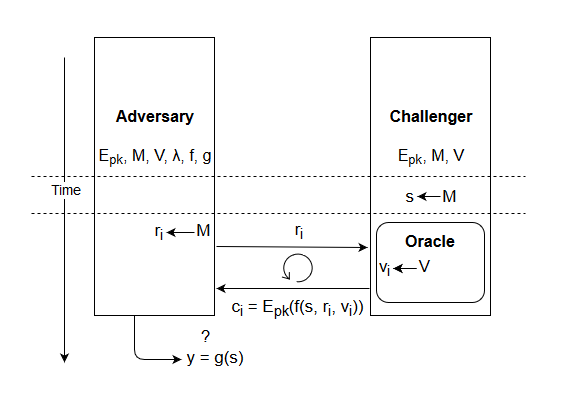
\includegraphics[width=0.48\textwidth]{reflection_game.png}
      \caption{Reflection Game}
   \end{figure}

\noindent {\bf Symmetric key version.}

The above game can be modified to deal with symmetric encryption. For this, the
choice of key is changed to be limited to a secret key instead of a public and
private key pair. The adversary is not given access to any key material.
Instead, the adversary is given access to an encryption oracle which encrypts a
given message using the secret key and returns the respective ciphertext, in
addition to the existing reflection oracle. Both oracles can be called an
arbitrary number of times by the challenger.

In the following proofs, we will assume that the game is played symmetrically.
As the attack does not pertain to the key exchange mechanism, all theorems can
be directly translated between the two versions of the game.

\section{The security of compression}\label{sec:comsec}

\subsection{The interdependence assumption}

Let $\bar{\mathcal{M}}$ be a joint distribution from which the random variables $(s, r)$
are drawn. We say that $s$ and $r$ are interdependent when:
\begin{equation*}
\begin{split}
\exists s_1, r_1, s_2, r_2:\\
\Pr_{(s, r) \leftarrow \bar{\mathcal{M}}}[(s, r) = (s_1, r_1)] < \Pr_{(s, r) \leftarrow \bar{\mathcal{M}}}[(s, r) = (s_2, r_1)]
\land\\
\Pr_{(s, r) \leftarrow \bar{\mathcal{M}}}[(s, r) = (s_1, r_2)] > \Pr_{(s, r) \leftarrow \bar{\mathcal{M}}}[(s, r) = (s_2, r_2)]
\end{split}
\end{equation*}

We observe that commonly compressed texts such as HTML content exhibit
interdependence almost everywhere. To be more precise, if we sample, for
example, digrams (two-letter sequences) in HTML content of popular websites and
treat this two-letter sequence $\phi = (s, r)$ of the two characters $s$ and
$r$ as a random variable $\phi$, we notice that $s$ and $r$ are dependent
variables and in fact interdependent. Similarly when sampling two-word sequences
$\phi = (s, r)$ of the two words $s$ and $r$ from English literature, then $s$
and $r$ are interdependent. The same occurs for digrams in English. This
straightforward fact is supported by extensive statistical analyses in the
scientific literature such as \cite{c18}.

The necessity of the assumption that the plaintext being compressed follows an
interdependent distribution will become clear shortly, when we introduce our
definition of compression functions.

\subsection{Compression idealness}

We now move on to define the notion of compression idealness.

Let $\mathcal{K}$ be a function from some input distribution $\bar{\mathcal{M}}$ to the
output space of all strings ${0, 1}^*$. $\mathcal{K}$ is an ideal compression
function when:
\begin{equation*}
\begin{split}
\forall w_1, w_2 \in \bar{\mathcal{M}}:\\
\Pr_{w \leftarrow \bar{\mathcal{M}}}[w = w_1] < \Pr_{w \leftarrow \bar{\mathcal{M}}}[w = w_2]
\iff\\
\lvert\mathcal{K}(w_1)\rvert > \lvert\mathcal{K}(w_2)\rvert
\end{split}
\end{equation*}

The intuitive notion behind compression idealness is that the encoding
function is somehow perfectly aware of the input distribution. It
exploits this knowledge of the input space to encode each possible
input in an ideal way – more often occurring plaintexts are compressed
better, i.e. in shorter length, than rarely occurring plaintexts.
Practical compression functions are not perfectly ideal, because the
distribution of plaintexts they try to cover is broad and ill-defined.
However, such compression functions try to learn the distribution of
the plaintext they are about to compress by observing frequencies of
occurrences and taking advantage of them.

We now turn our attention to two specific compression functions, the
LZ77 and Huffman function. These two compression functions are of
interest for two reasons. First, they are representative of the way
typical lossless compression functions work internally, by taking
advantage of letter frequencies (Huffman) or letter-sequence (LZ77)
repetitions. Second, they are the ones almost exclusively used in
practice. The DEFLATE algorithm, which is a composition of LZ77 and
Huffman, is the algorithm used in gzip, which is prevalent on the
modern web. In 2016, 98.85\% of websites that enabled compression used
some form of gzip \cite{c19}. We argue that both LZ77 and Huffman are nearly
ideal compression functions. The complexity of the Huffman and
especially the LZ77 algorithms arises from many intricate technical
details, such as, for instance, the sliding window size of LZ77. These
details make it impractical to deal with these functions in analytical
proofs. Hence, we support our idealness claims in an experimental
manner. For reference, the exact definitions of DEFLATE are given in
\cite{c12}.

\subsection{Composing with compression}\label{subsec:comcompose}

We now shift our interest to algorithms which compose compression and
encryption.  Therefore, we treat the public-key encryption scheme above as a
composition of a compression and encryption algorithm:
\begin{equation*}
    \mathcal{E} = Enc \circ Com
\end{equation*}

$Com$ denotes a compression function as defined above, while $Enc$ denotes an
encryption function. We stress our important assumption that $Enc$ is defined
on $\{0, 1\}^*$ and not on some fixed-length input.

\subsection{Length monotonicity}\label{subsec:lenmonotone}

An important assumption for our attack is that the encryption function $Enc$ is
\textit{length monotonic}. Specifically,
\begin{equation*}
\begin{split}
\forall m_1, m_2 \in \{0, 1\}^*\\
\forall \kappa_1, \kappa_2 \in \mathcal{K}\\
|m_2| > |m_1|
\Rightarrow
|Enc_{\kappa_1}(m_2)| \geq |Enc_{\kappa_2}(m_1)|
\end{split}
\end{equation*}

If the last inequality becomes strict, we call the encryption function
\textit{strictly length monotonic}.

A practical instance of a length monotonic encryption function is AES \cite{c8}.
Stream ciphers can be treated as strictly monotonic to the bit level.

\section{Compressibility with respect to predicates}\label{sec:propertycom}

Let $\mathcal{M}$ be a plaintext distribution and $Q(s)$ be a predicate on the
plaintext $s \in \mathcal{M}$. Let us use $\mathcal{M}_Q$ to denote the subset
of $\mathcal{M}$ restricted over the elements for which $Q$ holds
proportionally retaining measure and assuming $\mathcal{M}_Q \neq \emptyset$
and $\mathcal{M}_{\lnot Q} \neq \emptyset$.

For the specific property $Q$ and plaintext distribution $\mathcal{M}$, define:
\begin{equation*}
    \pi \defeq max(\Pr_{s \leftarrow \mathcal{M}}[Q(s)], 1 - \Pr_{s \leftarrow \mathcal{M}}[Q(s)])
\end{equation*}

Let $\mathcal{V}$ be a noise distribution from which a pair of noises
$\overbar{v} = (v_1, v_2) \leftarrow \mathcal{V}^2$ is drawn.  Let $\overbar{r}
= (r_1, r_2) \in \mathcal{M}^2$ be a reflection string pair, $Com$ be a
compression function, $f$ be a rendering function, and let $\alpha(\lambda)$ be
a non-negligible function.

We now examine how the lengths of compressing a secret $s$ rendered with
reflection strings $r_1$ and $r_2$ respectively compare.

The predicate $Q$ partitions the set $\mathcal{M}$ into two partitions
$\mathcal{M}_Q$ and $\mathcal{M}_{\lnot Q}$. We are interested in reflection
string pairs $\overbar{r} = (r_1, r_2)$ for which the comparison direction
depends on which partition $s$ belongs to.  The direction of comparison can
also depend on a noise vector $\overbar{v}$.  If $s \in \mathcal{M}_Q$, it
should compress better when reflection $r_1$ is used as compared to when $r_2$
is used. On the contrary, if $s \in \mathcal{M}_{\lnot Q}$, the opposite
direction should occur.  If this is the case for the selected reflection pair
and noise pair, we say that $Q$ compares favourably under $\overbar{r},
\overbar{v}$:
\begin{equation*}
\begin{split}
    cpr^Q_{f, Com}(s, \overbar{r}, \overbar{v})
    \defeq\\
    \begin{cases}
        |\mathcal{K}(s, r_1, v_1)| < |\mathcal{K}(s, r_2, v_2)| &\text{ if } Q(s)\\
        |\mathcal{K}(s, r_1, v_1)| > |\mathcal{K}(s, r_2, v_2)| &\text{ otherwise}
    \end{cases}
\end{split}
\end{equation*}

The reflection pair $\overbar{r}$ \textit{detects} predicate $Q$ under
compression $Com$ rendered with rendering function $f$ over the secret
distribution $\mathcal{M}$ and the noise distribution $\mathcal{V}$ when:
\begin{align*}
    dtc(Q, \overbar{r}, f, Com, \mathcal{M}, \mathcal{V})
    \defeq\\
    \exists \alpha \text{ non-negl}:\\
    \Pr_{s_1 \leftarrow \mathcal{M}_Q,
        s_2 \leftarrow \mathcal{M}_{\lnot Q},
        \overbar{v} \leftarrow \mathcal{V}^2}
        [cpr^Q_{f, Com}(s_1, \overbar{r}, \overbar{v}) \land
         cpr^Q_{f, Com}(s_2, \overbar{r}, \overbar{v})]
    \geq\\
    \pi + \alpha(\lambda)
\end{align*}

We call $Q$ \textit{compression-detectable} if a pair $\overbar{r}$ exists,
such that:
\begin{equation*}
    \exists \overbar{r} = r_1, r_2 \in \mathcal{M}:
    dct(Q, \overbar{r}, f, Com, \mathcal{M}, \mathcal{V})
\end{equation*}

Furthermore we require that such a pair $\overbar{r}$ is polynomially
computable:
\begin{align*}
    \exists \text{PPT } \mathcal{O}_R:\\
    dct(Q, \overbar{r}, f, Com, \mathcal{M}, \mathcal{V}),\\
    \overbar{r} \leftarrow \mathcal{O}_R(Com, f, Q, \mathcal{M}, \mathcal{V})
\end{align*}

The compression-detectability property exists in all common compression
functions as long as $s$ and $r$ compress in the same context. We will
illustrate such examples later in this work.

\section{Compression attacks}\label{sec:comattack}

\subsection{One-shot attack}

\begin{lemma}[Compression attack]

Let $Com$ be a compression function, $Enc$ be a strictly length-monotonic
encryption function, $f$ be a rendering function and $Q$ be a
compression-detectable plaintext predicate over plaintext distribution
$\mathcal{M}$ and noise distribution $\mathcal{V}$.

Then:
\begin{align*}
    \exists \alpha \text{ non-negl}:
    \forall Enc:
    \exists g:\\
    \exists PPT \mathcal{A}:
    \forall PPT \mathcal{S}:\\
    \text{Adv}_{\mathcal{SE}(Enc, Com), \mathcal{A}, \mathcal{S}}
    (\lambda, f, \mathcal{V}, \mathcal{M}, g) = \alpha(\lambda)
\end{align*}

\end{lemma}

\begin{IEEEproof}

Let $g$ be the boolean function $Q$ on the plaintext. Define the adversary
$\mathcal{A}$ as follows:

\begin{lstlisting}[texcl,mathescape,basicstyle=\small]
def $\mathcal{A}(Q, \mathcal{M}, y)$:
    $(r_1, r_2) \leftarrow \mathcal{O}_R(Com, f, Q, \mathcal{M}, \mathcal{V})$

    $l_1 = |\text{Reflect}^{\mathcal{E}_{pk}, \mathcal{V}}_s(r_1)|$
    $l_2 = |\text{Reflect}^{\mathcal{E}_{pk}, \mathcal{V}}_s(r_2)|$

    if $l_1 < l_2$:
        return True
    else:
        return False
\end{lstlisting}

Let $\mathcal{S}$ be an arbitrary simulator. Then we have:
\begin{align*}
    \Pr[\text{Game}_{\text{REF-SIM}}^{\mathcal{PE},\mathcal{S}}
        (\lambda, f, \mathcal{V}, \mathcal{M}, g) = 1] &=\\
    \Pr_{x \leftarrow \mathcal{M}, b \leftarrow \mathcal{S}(f, \mathcal{V}, \mathcal{M}, g)}
        [Q(x) = b]
\end{align*}

Letting the random variables $b$ and $x$:
\begin{align*}
    x &\leftarrow \mathcal{M}\\
    b &\leftarrow \mathcal{S}(f, \mathcal{V}, \mathcal{M}, g)
\end{align*}

Due to the independence of the simulator's output with the choice of $x$ we have:
\begin{align*}
    Pr[b = Q(x)] &=\\
    Pr[\lnot b|\lnot Q(x)]Pr[\lnot Q(x)] + Pr[b|Q(x)]Pr[Q(x)] &=\\
    Pr[\lnot b]Pr[\lnot Q(x)] + Pr[b]Pr[Q(x)] &=\\
    (1 - Pr[b])(1 - Pr[Q]) + Pr[b]Pr[Q(x)] &=\\
    1 - Pr[Q(x)] - Pr[b] + 2Pr[b]Pr[Q(x)]
\end{align*}

For a given $\Pr[Q]$, this function is monotonic in $\Pr[b]$ and therefore has
potential extrema at $\Pr[b] = 0$ or $\Pr[b] = 1$, for which cases the function
takes the values $1 - \Pr[Q(x)]$ and $\Pr[Q(x)]$ respectively. Therefore, the
maximum $\Pr[b]$ of the simulator is:
\begin{equation*}
    \Pr[Q(x) = b] = max(\Pr[Q(x)], 1 - \Pr[Q(x)]) = \pi
\end{equation*}

And therefore:
\begin{align*}
    \forall \mathcal{S}:\\
    \Pr[
        \text{Game}_{\text{REF-SIM}}^{\mathcal{PE},\mathcal{S}}
        (\lambda, f, \mathcal{V}, \mathcal{M}, g) = 1
    ]
    \leq\\
    max(Pr[Q(x)], 1 - Pr[Q(x)])
\end{align*}

From the compression detectability of Q we know that:
\begin{align*}
    \exists \alpha \text{ non-negl}:\\
    \Pr_{s_1 \leftarrow \mathcal{M}_Q,
         s_2 \leftarrow \mathcal{M}_{\lnot Q},
         \overbar{v} \leftarrow \mathcal{V}^2}
         [cpr^Q_{f, Com}(s_1, \overbar{r}, \overbar{v}) \land
          cpr^Q_{f, Com}(s_2, \overbar{r}, \overbar{v})]
    \geq\\
    \pi + \alpha(\lambda)
\end{align*}

Therefore:
\begin{align*}
    \Pr_{s_1 \leftarrow \mathcal{M}_Q,
         \overbar{v} \leftarrow \mathcal{V}^2}
         [cpr^Q_{f, Com}(s_1, \overbar{r}, \overbar{v})]
    \geq
    \pi + \alpha(\lambda) \land\\
    \Pr_{s_2 \leftarrow \mathcal{M}_{\lnot Q},
         \overbar{v} \leftarrow \mathcal{V}^2}
         [cpr^Q_{f, Com}(s_2, \overbar{r}, \overbar{v})]
    \geq
    \pi + \alpha(\lambda)
\end{align*}

And so:
\begin{align*}
    \Pr_{s \leftarrow \mathcal{M},
         \overbar{v} \leftarrow \mathcal{V}^2}
         [cpr^Q_{f, Com}(s, \overbar{r}, \overbar{v})]
    =\\
    \Pr[cpr^Q_{f, Com}(s, \overbar{r}, \overbar{v})|Q(s)]\Pr[Q(s)]
    +\\
    \Pr[cpr^Q_{f, Com}(s, \overbar{r}, \overbar{v})|\lnot Q(s)]\Pr[\lnot Q(s)]
    \geq\\
    (\pi + \alpha(\lambda))(\Pr[Q(s)] + (1 - \Pr[Q(s)))
    =\\
    \pi + \alpha(\lambda)
\end{align*}

Let us now examine the event of $\mathcal{A}$ being successful, denoted Succ,
when $cpr^Q_{f, Com}(s, \overbar{r}, \overbar{v})$. Assuming $Q(s)$:
\begin{align*}
    \Pr[|\mathcal{K}(s, r_1, v_1)| < |\mathcal{K}(s, r_2, v_2)||Q(s)]
    = \pi + \alpha(\lambda)
\end{align*}

And from the strict length monotonicity of $Enc$ it follows that:
\begin{align*}
    \Pr[&|Enc(\mathcal{K}(s, r_1, v_1))| <\\&|Enc(\mathcal{K}(s, r_2, v_2))||Q(s)]
        \geq \pi + \alpha(\lambda)\\
    \Rightarrow \Pr[&
        |\text{Reflect}^{\mathcal{E}_{pk}, \mathcal{V}}_s(r_1)|
        <
        |\text{Reflect}^{\mathcal{E}_{pk}, \mathcal{V}}_s(r_2)||Q(s)
    ]
        \geq \pi + \alpha(\lambda)\\
    \Rightarrow \Pr[&l_1 < l_2|Q(s)]
        \geq \pi + \alpha(\lambda)\\
    \Rightarrow \Pr[&\text{Succ}|Q(s)]
        \geq \pi + \alpha(\lambda)\\
\end{align*}

The case for $\lnot Q(s)$ is the same, but with a different inequality direction:
\begin{align*}
    \Pr[|\mathcal{K}(s, r_1, v_1)| > |\mathcal{K}(s, r_2, v_2)||\lnot Q(s)]
        \geq\\
        \pi + \alpha(\lambda)\\
    \Rightarrow \Pr[\text{Succ}|\lnot Q(s)] \geq\\
    \pi + \alpha(\lambda)\\
\end{align*}

And so the probability of success is given:
\begin{align*}
    \Pr[\text{Succ}] =\\
    \Pr[\text{Succ}|Q(s)]\Pr[Q(s)]
    +
    \Pr[\text{Succ}|\lnot Q(s)]\Pr[\lnot Q(s)] \geq\\
    \pi + \alpha(\lambda)
\end{align*}

Therefore,
\begin{align*}
    \forall PPT \mathcal{S}:
    \text{Adv}_{\mathcal{SE}(Enc, Com), \mathcal{A}, \mathcal{S}}
        (\lambda, f, \mathcal{V}, \mathcal{M}, g)
    \geq\\
    |\pi + \alpha(\lambda) - \pi| = \alpha(\lambda)
\end{align*}

Which is non-negligible.

\end{IEEEproof}

\subsection{Amplified attack}

We can now amplify the attack to achieve a better probability of success by a small modification in our adversary.
The amplification is parameterized by an odd parameter $k$.

Let the amplification adversary be defined as follows:

\begin{lstlisting}[texcl,mathescape,basicstyle=\small]
def $\mathcal{A}(Q, \mathcal{M})$:
    $(r_1, r_2) \leftarrow \mathcal{O}_R(Com, f, Q, \mathcal{M}, \mathcal{V})$

    $low = 0$
    $high = 0$

    for $i$ = $0$ to $k$:
        $l_1 = |\text{Reflect}^{\mathcal{E}_{pk}, \mathcal{V}}_s(r_1)|$
        $l_2 = |\text{Reflect}^{\mathcal{E}_{pk}, \mathcal{V}}_s(r_2)|$

        if $l_1 < l_2$:
            $low = low + 1$
        else:
            $high = high + 1$

    if $low > high$:
        return True
    else:
        return False
\end{lstlisting}

\begin{lemma}[Amplification]

Under the assumptions of the Compression Attack Theorem against $f, Com$
and compression-detectable predicate $Q$ with non-negligible
detectability margin $\alpha(\lambda)$,
the amplified adversary achieves an arbitrarily large advantage
against a non-negligible subset of elements, the
\textit{amplifiable elements} distinguished by predicate $Amp$.
\begin{align*}
    \forall Enc:
    \exists g:\\
    \exists PPT \mathcal{A}:
    \forall PPT \mathcal{S}:\\
    \exists Amp:
    \exists B \text{ non-negl}:
    \exists C \text{ negl}:\\
    \Pr_{s \leftarrow \mathcal{M}}[Amp(s)] = B(\lambda) \land\\
    \text{Adv}_{\mathcal{SE}(Enc, Com), \mathcal{A}, \mathcal{S}_{Amp}}
    (\lambda, f, \mathcal{V}, \mathcal{M}, g) = 1 - \pi - C(k)
\end{align*}

\end{lemma}

\begin{IEEEproof}

From the fact that $Q$ is compression-detectable and from the Compression Attack Theorem, we have that:
\begin{align*}
    \Pr_{s \leftarrow \mathcal{M},
         \overbar{v} \leftarrow \mathcal{V}^2}
         [cpr^Q_{f, Com}(s, \overbar{r}, \overbar{v})]
    =\\
    \pi + \alpha(\lambda)
\end{align*}

Some elements $s \in \mathcal{M}$ allow for better compression-detectability than others under the fixed
reflection vector $\overbar{r}$. Call these elements \textit{amplifiable} and define predicate:
\begin{align*}
    Amp(s) \defeq
    \Pr_{\overbar{v} \leftarrow \mathcal{V}^2}
    [cpr^Q_{f, Com}
     (s, \overbar{r}, \overbar{v})]
    \geq
    \frac{1}{2} + \frac{\alpha(\lambda)}{2}
\end{align*}

We will now obtain a lower bound on the probability of an element being amplifiable.

Let:

% B derivation: (where \beta(\lambda) = \alpha(\lambda) / 2)
% B + (\frac{1}{2} + \alpha(\lambda)/2)(1 - B) = \pi + \alpha(\lambda)
% B + \frac{1}{2} + \alpha(\lambda)/2 - B(\frac{1}{2} + \beta(\lambda)) = \pi + \alpha(\lambda)
% \frac{1}{2} + \beta(\lambda) + B(\frac{1}{2} - \beta(\lambda)) = \pi + \alpha(\lambda)
% B(\frac{1}{2} - \beta(\lambda)) = \pi + \alpha(\lambda) - \frac{1}{2} - \beta(\lambda)
% B = (\pi + \alpha(\lambda) - \frac{1}{2} - \beta(\lambda)) / (\frac{1}{2} - \beta(\lambda))
% B = (\pi + \alpha(\lambda) - \frac{1}{2} - \frac{\alpha(\lambda)}{2}) / (\frac{1}{2} - \frac{\alpha(\lambda)}{2})
% B = (\pi - \frac{1}{2} + \frac{\alpha(\lambda)}{2}) / (\frac{1}{2} - \frac{\alpha(\lambda)}{2})
% B = \pi / (\frac{1}{2} - \frac{\alpha(\lambda)}{2}) - (\frac{1}{2} - \frac{\alpha(\lambda)}{2}) / (\frac{1}{2} - \frac{\alpha(\lambda)}{2})
% B = \pi / (\frac{1}{2} - \frac{\alpha(\lambda)}{2}) - 1
\begin{align*}
    B = \frac{\pi}{\frac{1}{2} - \frac{\alpha(\lambda)}{2}} - 1
\end{align*}

$B$ is non-negligible in $\lambda$.

Assume, for the sake of contradiction, that:
\begin{align*}
    \Pr_{s \leftarrow \mathcal{M}}
    [Amp(s)] < B
\end{align*}

Then we have:
\begin{align*}
    \Pr_{s \leftarrow \mathcal{M},
         \overbar{v} \leftarrow \mathcal{V}^2}
         [cpr^Q_{f, Com}(s, \overbar{r}, \overbar{v})]
    =\\
    \Pr_{s \leftarrow \mathcal{M},
         \overbar{v} \leftarrow \mathcal{V}^2}
         [cpr^Q_{f, Com}(s, \overbar{r}, \overbar{v})|Amp(s)]\Pr[Amp(s)]
    +\\
    \Pr_{s \leftarrow \mathcal{M},
         \overbar{v} \leftarrow \mathcal{V}^2}
         [cpr^Q_{f, Com}(s, \overbar{r}, \overbar{v})|\lnot Amp(s)]\Pr[\lnot Amp(s)]
    <\\
    B + (\frac{1}{2} + \frac{\alpha}{2})(1 - B)
\end{align*}

But then:
\begin{align*}
    B + (\frac{1}{2} + \frac{\alpha(\lambda)}{2})(1 - B) =
    \pi + \alpha(\lambda)
\end{align*}

And this contradicts the assumption that $Q$ is compression-detectable. Therefore:
\begin{align*}
    \Pr_{s \leftarrow \mathcal{M}}
    [Amp(s)] \geq B
\end{align*}

It remains to show that the advantage of the adversary can be
arbitrarily large, i.e. that for some negligible $C$ we have:
\begin{align*}
    \text{Adv}_{\mathcal{SE}(Enc, Com), \mathcal{A}, \mathcal{S}_{Amp}}
    (\lambda, f, \mathcal{V}, \mathcal{M}, g) = 1 - \pi - C
\end{align*}

Indeed, observe that the amplifying adversary performs a repeated Bernoulli
trial with $k$ repetitions and extracts a majority. Let $X$ be the number of
repetitions that are successful for the adversary. Letting $\overbar{v}_i$
be the noise chosen from $\mathcal{V}^2$ during the $i$-th round, $X$ is defined:
\begin{align*}
    X \defeq |\{ i: cpr^Q_{f, Com}(s, \overbar{r}, \overbar{v}_i) \}|
\end{align*}

$X$ follows the binomial distribution, and therefore its expected value is:
\begin{align*}
    E[X] = \frac{k}{2} + \frac{\alpha k}{2}
\end{align*}

Let Succ denote the event of the amplified adversary succeeding. Then Succ
is equivalent to $X > \frac{k}{2}$.

Because $\alpha$ is non-negligible and due to the tail bounds of the binomial
distribution, we have:
\begin{align*}
    Pr[Succ] = 1 - C(k)
\end{align*}

Where $C$ is a negligible function.
\end{IEEEproof}

\section{Defense}\label{sec:defense}
We propose a defense, \textit{context hiding}, that mitigates a class of
practical compression side-channel attacks such as CRIME, TIME, BREACH, Rupture,
and HEIST. The full plaintext recovery these attacks perform is no longer
possible when our defense is applied.

Context hiding is built on the premise of separating secrets in a per-origin
manner in order to avoid cross-compression. In order to achieve this we define
what constitutes an origin and what properties same-origin secrets share. This
section describes the key components of the defense and the code implementation.

\subsection{Context hiding properties}

\subsubsection{Origins}
An origin is a uniquely identifiable party that generates content. A party can
be either a physical entity, like a user, or an application that provides a
service. It is important to properly identify the party that generated, or could
have generated, a piece of content. The definition of origins should reflect the
ability to generate all content that is assigned to each origin.

\subsubsection{Same-origin secrets}
Defining origins is the first step to identifying same-origin secrets. Secrets
are content pieces that are assinged to origins. Secrets that are assigned to an
origin should have been generated by the party that this origin identifies.
Also the origin's party has access to all content in this origin. This results
in a secret $a$ being insecure for all other secrets belonging in $a$'s origin.

\subsection{Context hiding functionality}
Our defense method proposes disabling cross-compression by applying a simple
substitution cipher derived from a random permutation of the plaintext alphabet.

Firstly, we identify the origins based on the output $m$ of rendering function
$f$ and store them in array $origins$. Each secret $s_i$ in $m$ is then
separated based on its origin. Each origin is uniquely identified by an integer
in range $[0, |origins|-1)$.

Secondly, we identify the alphabet for each origin. An origin's alphabet
consists of all possible characters that a secret of this origin may contain.
For each origin, we generate a random permutation of the origin's alphabet and
store it in the array $permutations$. The first element in the $permutations$
array corresponds to the first origin in the $origins$ array and so forth.

In order to secure a secret $s$ we apply a hiding function. The hiding function
\textit{hide} takes two arguments, the secret $s$ and the permutation $p$ of the
secret's origin. It applies the substitution cipher on each character in $s$ and
returns the permuted secret $s'$.

\begin{lstlisting}[texcl,mathescape,basicstyle=\small]
def hide($s, p$):
    $s' = ''$
    for $ch \in s$:
        $s' = s' || Permute_p(ch)$
    return $s'$
\end{lstlisting}

The protected secret $s'$ is annotated by the special characters
$\beta_{start}^i$, $\beta_{end}^i$ that mark the start and the end of any
substring that needs to be unpermuted.

The output $m'$ that is produced after hiding all secrets includes the
permutation array $permutations$, so that applying the reverse permutation on
all secrets is possible.

The permuted secrets in $m'$ can be retrieved using the special annotation
characters $\beta_{start}^i$ and $\beta_{end}^i$ that are unique per origin.

The initial secret $s$ can be retrieved from the protected secret $s'$
using the \textit{unhide} function. This function takes secret $s'$ and
permutation $p$ of the secret's origin and applies the reverse permutation on
$s'$, returning the unpermuted secret $s$.

\begin{lstlisting}[texcl,mathescape,basicstyle=\small]
def unhide($s', p$):
    $s = ''$
    for $ch \in s'$:
        $s = s || Unpermute_p(ch)$
    return $s$
\end{lstlisting}

\subsection{The CTX defense}\label{subsec:ctx}

\subsubsection{Implementation}
Our contributions include the development of the CTX defense. CTX is an
implementation of the context hiding method described in the previous section
for HTML web pages.

It is up to the application developer to decide which portions of the response
are sensitive and must be protected as secrets. Sensitive data does not only
include high-value secrets such as passwords and CSRF tokens, but also user data
that the developer wishes to keep private. Some examples are the bodies of email
messages in Gmail, the chat messages received or sent to a friend on Facebook,
the contents of documents and spreadsheets in Google Docs and the list of online
friends on Facebook or Google Hangouts, as they contain all the important
contacts of the victim. Practically any piece of information which is only
accessible when logged in is potentially a secret and should be CTX protected.
On the other hand, some data do not typically need compression-security
protection, e.g. static HTML portions that are accessible on a website even when
logged out.

The minimum amount of origins is one origin for the entire response, in which
case CTX is not protecting any part of the plaintext, and the maximum is one
origin per character. The latter would result in the best possible security
under CTX, although compression would be effectively disabled possibly resulting
in poor performance. This is the case with defenses such as secret masking.

Different-origin secrets are then forced to compress separately, i.e. not
cross-compress. However, compression is achieved within each context. The
default origin alphabet is ASCII characters (0 - 128). In order to randomly
permute the secret alphabet, we use the Fisher--Yates shuffle
algorithm~\cite{c17}.

Secrets are then permuted by the server using the generated permutation of the
corresponding origin prior to TLS encryption and network transmission. Upon
arrival on the client side, the inverse permutation is applied to decode the
secret. The same permutation is applied to all secrets of the same origin. That
way, better compression is achieved intra-origin.

Each time the server issues an HTTPS response, new per-origin permutations are
generated. The power of the BREACH attack lies to the assumption that we can
perform multiple requests to the target website while the transmitted secret
remains the same. Since new alphabet permutations are generated per HTTPS
response, the statistical analysis performed by Rupture is no longer feasible.

\subsubsection{A detailed example}

Each time CTX protects a secret, three parameters need be defined: the secret,
the origin, and the permutation alphabet. In our example we will use the
permutation alphabet of ASCII printable characters, which consist of ASCII codes
9-13 and 32-126.

The first secret that needs to be protected is the string "secret1" which is
generated by the origin "testsorigin1". In order to protect this secret, CTX
will generate a random permutation of ASCII printable characters. Each character
in the permutation corresponds to a single ASCII printable character, so that
the first character in the permutation corresponds to ASCII 9 and the last to
ASCII 126. CTX will then apply the permutation on the secret. Suppose that the
correspondence of printable-permutation characters is:

\begin{description}
    \item{$\cdot$ s} $\rightarrow$ 0
    \item{$\cdot$ e} $\rightarrow$ f
    \item{$\cdot$ c} $\rightarrow$ )
    \item{$\cdot$ r} $\rightarrow$ 4
    \item{$\cdot$ t} $\rightarrow$ *
    \item{$\cdot$ 1} $\rightarrow$ l
    \item (...)
\end{description}

The permuted secret will then be "0f)40*l".

A second secret is the string "secret2" from origin "testorigin2". Following the
same procedure, CTX will generate a permutation which is described as follows:

\begin{description}
    \item{$\cdot$ s} $\rightarrow$ t
    \item{$\cdot$ e} $\rightarrow$ 9
    \item{$\cdot$ c} $\rightarrow$ (
    \item{$\cdot$ r} $\rightarrow$ l
    \item{$\cdot$ t} $\rightarrow$ j
    \item{$\cdot$ 2} $\rightarrow$ 2
    \item (...)
\end{description}

The second permuted secret will then be "t9(l9j2".

Permutations are randomly generated per origin, so the two permutations for
"testorigin1" and "testorigin2" are not dependent and each is needed in order to
reverse permute the corresponding secret.

\subsubsection{Experimental results}

We have conducted several experiments to evaluate the performance of web
services protected by CTX. The results of these experiments are overwhelmingly
positive and should be taken into account when considering incorporating CTX in
a web service.

The CTX parameters that affect performance are basically 3: the number of
origins, the total amount of plaintext response, and the amount of secrets in
the response. Each parameter affects the performance differently and will be
examined thoroughly in the following sections.

Our experiments focused on each parameter separately, so the results reflect the
performace under each one independently. A combination of the parameters may
result in slightly different results when used in real-world systems.

In all our tests we use an HTML web page where the secrets are strings of
English literature. The tests measure the performance penalty in terms of size
overhead in the compressed response HTML. The penalty in execution time is
considered insignificant and not included when less than 10ms.

The first parameter, the number of origins, mainly affects the compression
performance of the secrets. The more origins are used the bigger the response,
both compressed and uncompressed, will be. This is expected, given the fact that
secrets from different origins do not cross-compress.

Our experiment covered a 650KB web page, which consists of 1\% secrets and 99\%
static data. The secrets are distributed in origins that range from 1 to 50, so
the length of a secret per origin is reduced as origins increase and the total
amount of secrets and static data remains the same.

   \begin{figure}[thpb]
      \centering
      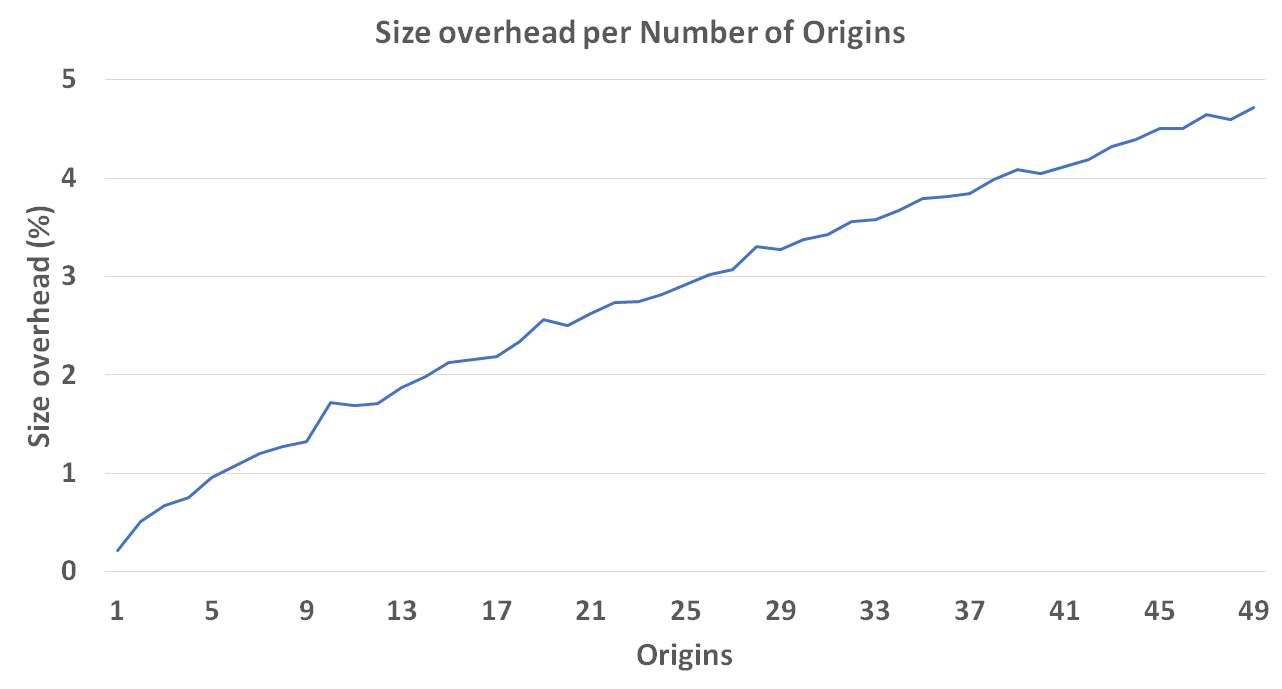
\includegraphics[width=0.48\textwidth]{experiments/origins.png}
      \caption{Origins}
   \end{figure}

As figure 2 shows, the size overhead when 1 origin is used is less than 0.5\%
and about 4.7\% when 49 origins are used. This means that the compressed
response when CTX is used is expected to be 1.47x the unprotected compressed
response when 50 origins are used. In comparison, disabling compression would
result in 976.8\% overhead.

The second parameter, the total response size, affects the impact of CTX on the
compressed response.

In this case, we use 50 origins which relate to equal parts of 1\% of the total
response. The total response ranges from a 13KB to a 650KB web page. Our
experiments show that CTX adds a consistent amount of bytes in the compressed
response, between 5-7KB. This results in a significant performance increase for
small web pages, which becomes less observable as the web page grows larger.

   \begin{figure}[thpb]
      \centering
      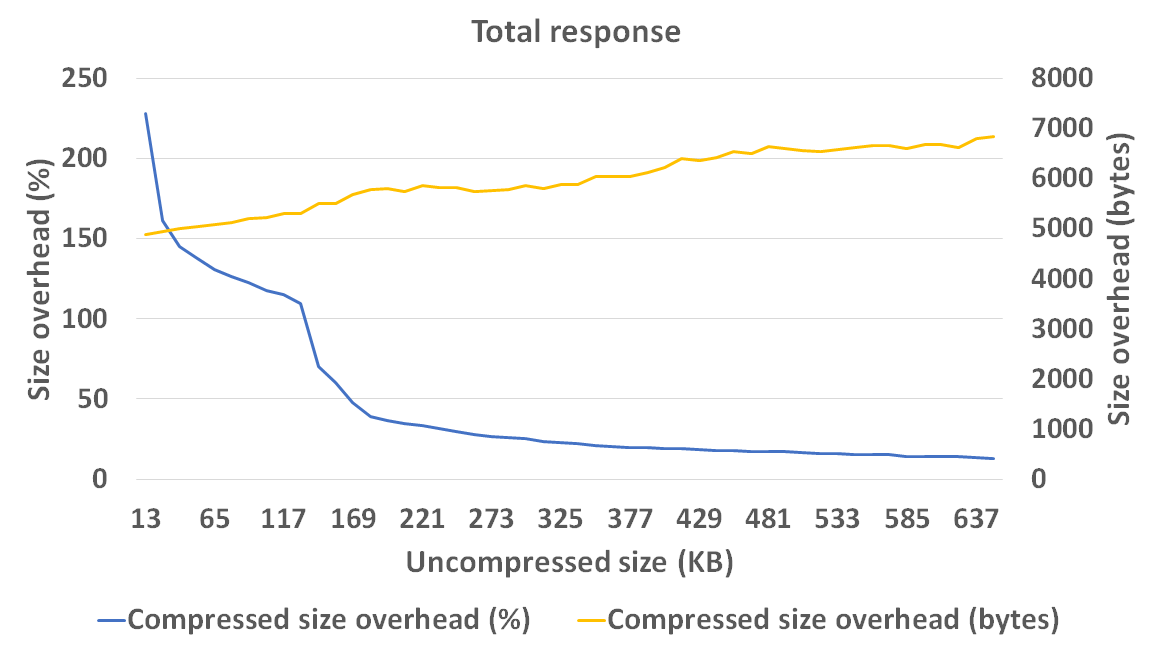
\includegraphics[width=0.48\textwidth]{experiments/total_response.png}
      \caption{Total response}
   \end{figure}

Figure 3 depicts the results of this experiment. A 13KB web page suffers a 5KB
CTX overhead, which corresponds to 228\% increase in compressed response. On the
other hand, CTX will add only 7KB of compressed data for a 650KB web page, which
results in a 12\% increase.  Disabling compression entirely would add overhead
that ranges from 500\% to 91\% for the tested web pages.

The third parameter is the total amount of secrets in the response. In our
example we use a 650KB web page with 50 CTX origins. The secrets range from 1\%
up to 50\% of the web page, the rest being static data, and are evenly
distributed across origins.

   \begin{figure}[thpb]
      \centering
      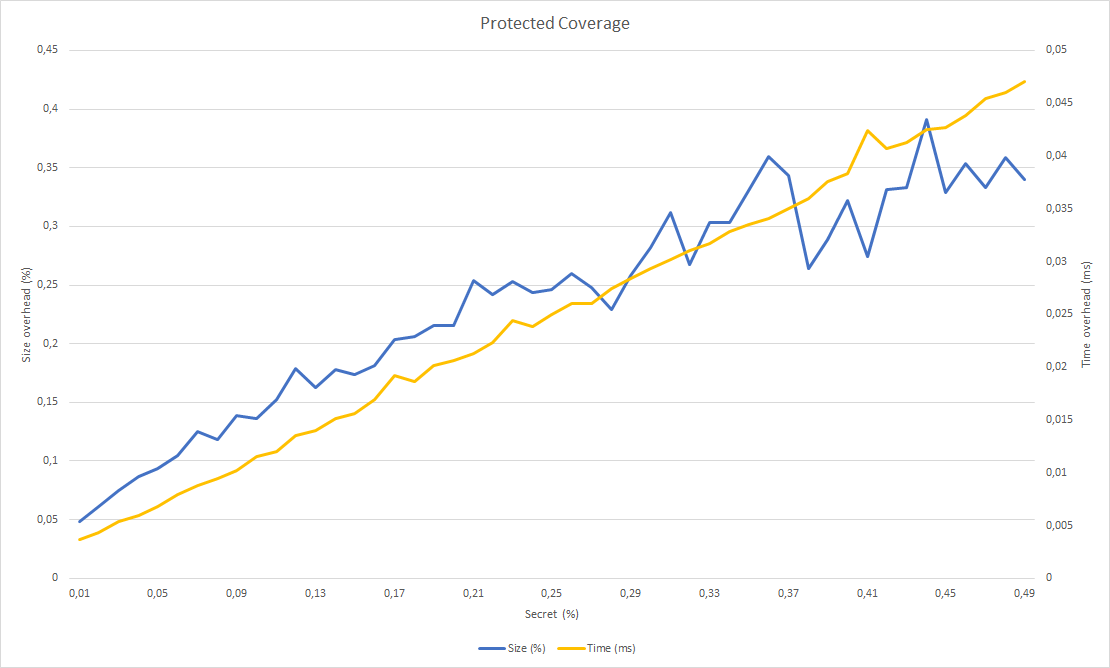
\includegraphics[width=0.48\textwidth]{experiments/response_secrets.png}
      \caption{Response secrets}
   \end{figure}

Figure 4 shows the results in this case. We find that protecting 1\% of the
tested web page results in less than 5\% size overhead, whereas protecting 50\% of
the page results in 35\%. This test also showed a noteworthy time increase in
execution time, where for 10\% secrets in the web page CTX adds 10ms of
execution time, while for 50\% it adds 47ms.

However, it should be noted that our tests are particularly strict. A typical
website response consists mainly of HTML code or libraries that usually need not
be protected. In this case, the amount of secrets in the response would not
exceed 1\% of the total response, in which case the CTX overhead as shown by our
experiments is totally acceptable. For example, Facebook and Gmail typically
only need protect approximately 0.5\% of the response.

In comparison, disabling compression would again result in 976.8\% load overhead
and a network transmittion time overhead that, depending on the client's and the
server's network, may be several seconds.

\section{Application}\label{sec:application}

BREACH is an example of a side-channel attack, that uses reflection in
order to steal plaintext compressed and encrypted in the web.

\subsection{BREACH as a compression distinguishing
attack}\label{subsec:breachapp}
BREACH is an instance of the attack model described in \ref{sec:comattack}.

A secret is defined as any string in the response plaintext of a web page, such
as authentication tokens, private messages etc.

The property $g$ of the secret that is being compromised is defined as: "What is
the prefix $p$ of secret $s$, given a known prefix $p_s$, where $|p| - |p_s| =
1$?".

The distribution $\mathcal{M}$ is ${p_s:t}$, where $t \in \mathcal{S}$ and
$\mathcal{S}$ is a known alphabet of ASCII symbols.

The rendering function $f$ is the website response code rendering function. This
function concatenates secret $s$ with static strings $u$, noise $v$ and the
reflection string $r$.

The compression function is gzip, which implements the DEFLATE algorithm
\cite{c12}, that is the combination of LZ77 and Huffman coding.

The encryption function is any encryption algorithm used in communications over
the Internet, most notably AES.

The web application that is being attacked with BREACH offers an endpoint that
allows requests via HTTP GET, where an HTTP GET parameter is included in the
response. This endpoint constitutes the reflection oracle.

The adversary should be able to issue requests to the given endpoint and monitor
the traffic from and to the attacking browser. At this point, the adversary can
issue requests on different elements of $\mathcal{S}$ and compare the response lengths. As
long as a difference in lengths across different requests is noticeable, the
compression distinguishing attack is successful.

\subsection{Rupture implementation}\label{subsec:rupture}
Our contributions include the development development of a production-grade
framework for implementing this class of attacks called Rupture \cite{c13}.
Rupture was developed as part of the work on extending the BREACH attack against
modern systems and block ciphers and was first discussed as an attack mechanism
in \cite{c7}.

As long as a vulnerable endpoint described in \ref{sec:comattack} is found,
Rupture offers the ability to inject malicious code in any computer in the
network. This code would issue requests to the endpoint and serve as a caller of
the reflection oracle that is the endpoint.

Furthermore, it enables the traffic inspection and analysis of packet
lengths. Encrypted network packets serve as the response $c_i$ from the
reflection oracle and the length of each packet is visible on the network and
captured.

In addition, Rupture offers multiple instances of oracle $\mathcal{O}_R$, based
on various $Q$ described in \ref{subsec:parallel}, and enables the automated
computation of the reflection strings in each stage of the attack.

Finally, it amplifies the attack by issuing multiple requests per candidate
symbol in alphabet $\mathcal{S}$ in order to demonstrate better probability of
success. This is achieved by grouping requests in samplesets, where each
sampleset contains requests on a symbol in alphabet $\mathcal{S}$. Requests in a
sampleset may be constructed to enable optimization methods described in
\ref{subsec:blockalign} and \ref{subsec:parallel}.

Rupture issues the attack in rounds. Each round consists of phases, whose result
leads to the detection of property $Q$, where $Q$ is specified by the method of
attack described in \ref{subsec:parallel}, with some confidence $n$. Confidence
is a metric calculated in bytes, that depicts the length difference between a
pair $r_1, r_2$ of requests that make property $Q$ of secret $s$ compression
detectable.

\subsection{Rupture architecture}\label{app:rupture}
Rupture consists of multiple components that collaborate in executing
compression-based attacks, such as BREACH. Each component is autonomous and
communicates with the rest over the network.

\subsubsection{Client}

The client component is a Javascript code that issues requests towards a chosen
endpoint. This endpoint should offer the functionality described in
\ref{subsec:breachapp} and serve as the reflection oracle of the attack. The client
needs to be executed from the browser of the victim that the adversary is trying
to steal secrets from. That way, the victim's authentication cookies will be
included in the request and lead to the endpoint including secrets in the
response.

The client contains minimal logic. It connects to the real-time service through
a command-and-control channel and registers itself there. Afterwards, it waits
for work instructions by the command-and-control channel, which it executes. The
client does not take any decisions or receive data about the progress of the
attack other than the work it is requested to do. This is intentional so as
to conceal the workings of the adversary analysis mechanisms from the victim
in case the victim attempts to reverse engineer what the adversary is doing.
Furthermore, it allows the system to be upgraded without having to deploy a
new client at the victim's network, which can be a difficult process.

As a regular user is browsing the Internet, multiple clients will be
injected in insecure pages and they will run under various contexts. All of
them will register and maintain an open connection through a
command-and-control channel with the real-time service. The real-time
service will enable one of them for this victim, while keeping the others
dormant. The one enabled will then receive work instructions to perform the
required requests. If the enabled client dies for whatever reason, such as a
closed tab, one of the rest of the clients will be waken up to take over the
attack.

\subsubsection{Injector}

The injector component is responsible for injecting code to the victim's
computer for execution. The injection is performed by ARP spoofing the local
network and forwarding all traffic in a Man-in-the-Middle manner. Since all HTTP
responses are infected, this provides for greatly increased robustness.

The injector component needs to run on the victim network and as such is
light-weight and stateless. It can easily be deployed on a small machine and
used for massive attacks. Multiple injectors can be deployed to different
networks, all controlled by the same central command-and-control channel.

\subsubsection{Realtime}

The realtime service is a service which awaits for work requests by clients. It
can handle multiple targets and victims. It receives command-and-control
connections from various clients which can live on different networks,
orchestrates them, and tells them which ones will remain dormant and which ones
will receive work, enabling one client per victim.

It maintains open web socket command-and-control connections with clients and
connects to the backend service, facilitating the communication between the two.

\subsubsection{Sniffer}

The sniffer component is responsible for collecting data directly from the
victim's network. As the client issues chosen plaintext requests, the sniffer
collects the respective ciphertext requests and ciphertext responses as they
travel on the network. These encrypted data are then transmitted to the backend
for further analysis and decryption.

The sniffer component has access to the victim's network traffic and
keeps track of the encrypted communication between the victim and the endpoint.
The length of the packets is unencrypted, so the sniffer is able to collenct and
report the observations on the network to the backend component.

The sniffer exposes an HTTP API which is utilized by the backend for controlling
when sniffing starts, when it is completed, and to retrieve the data that was
sniffed.

\subsubsection{Backend}

The backend component is a Python code that controls the attack execution. It
initializes the attack and calculates the initial request sets that should be
collected. It is responsible for strategic decision taking, statistical
analysis of samples collected, adaptively advancing the attack, and storing
persistent data about the attacks in progress for future analysis.

It communicates with the realtime component in order to guide the client as to
what requests need to be made at each stage of the attack. Meanwhile, it orders
the sniffer to listen and report network traffic, which is collected and stored
at the end of each phase of the attack. At each round, the backend analyzes the
sniffer reports and calculates the probability of success for the attack. At the
end of each round, property $Q$, which depends on the method of attack described
in \ref{subsec:reflectionmethods}, is detected, until the entire secret is
calculated.

   \begin{figure}[thpb]
      \centering
      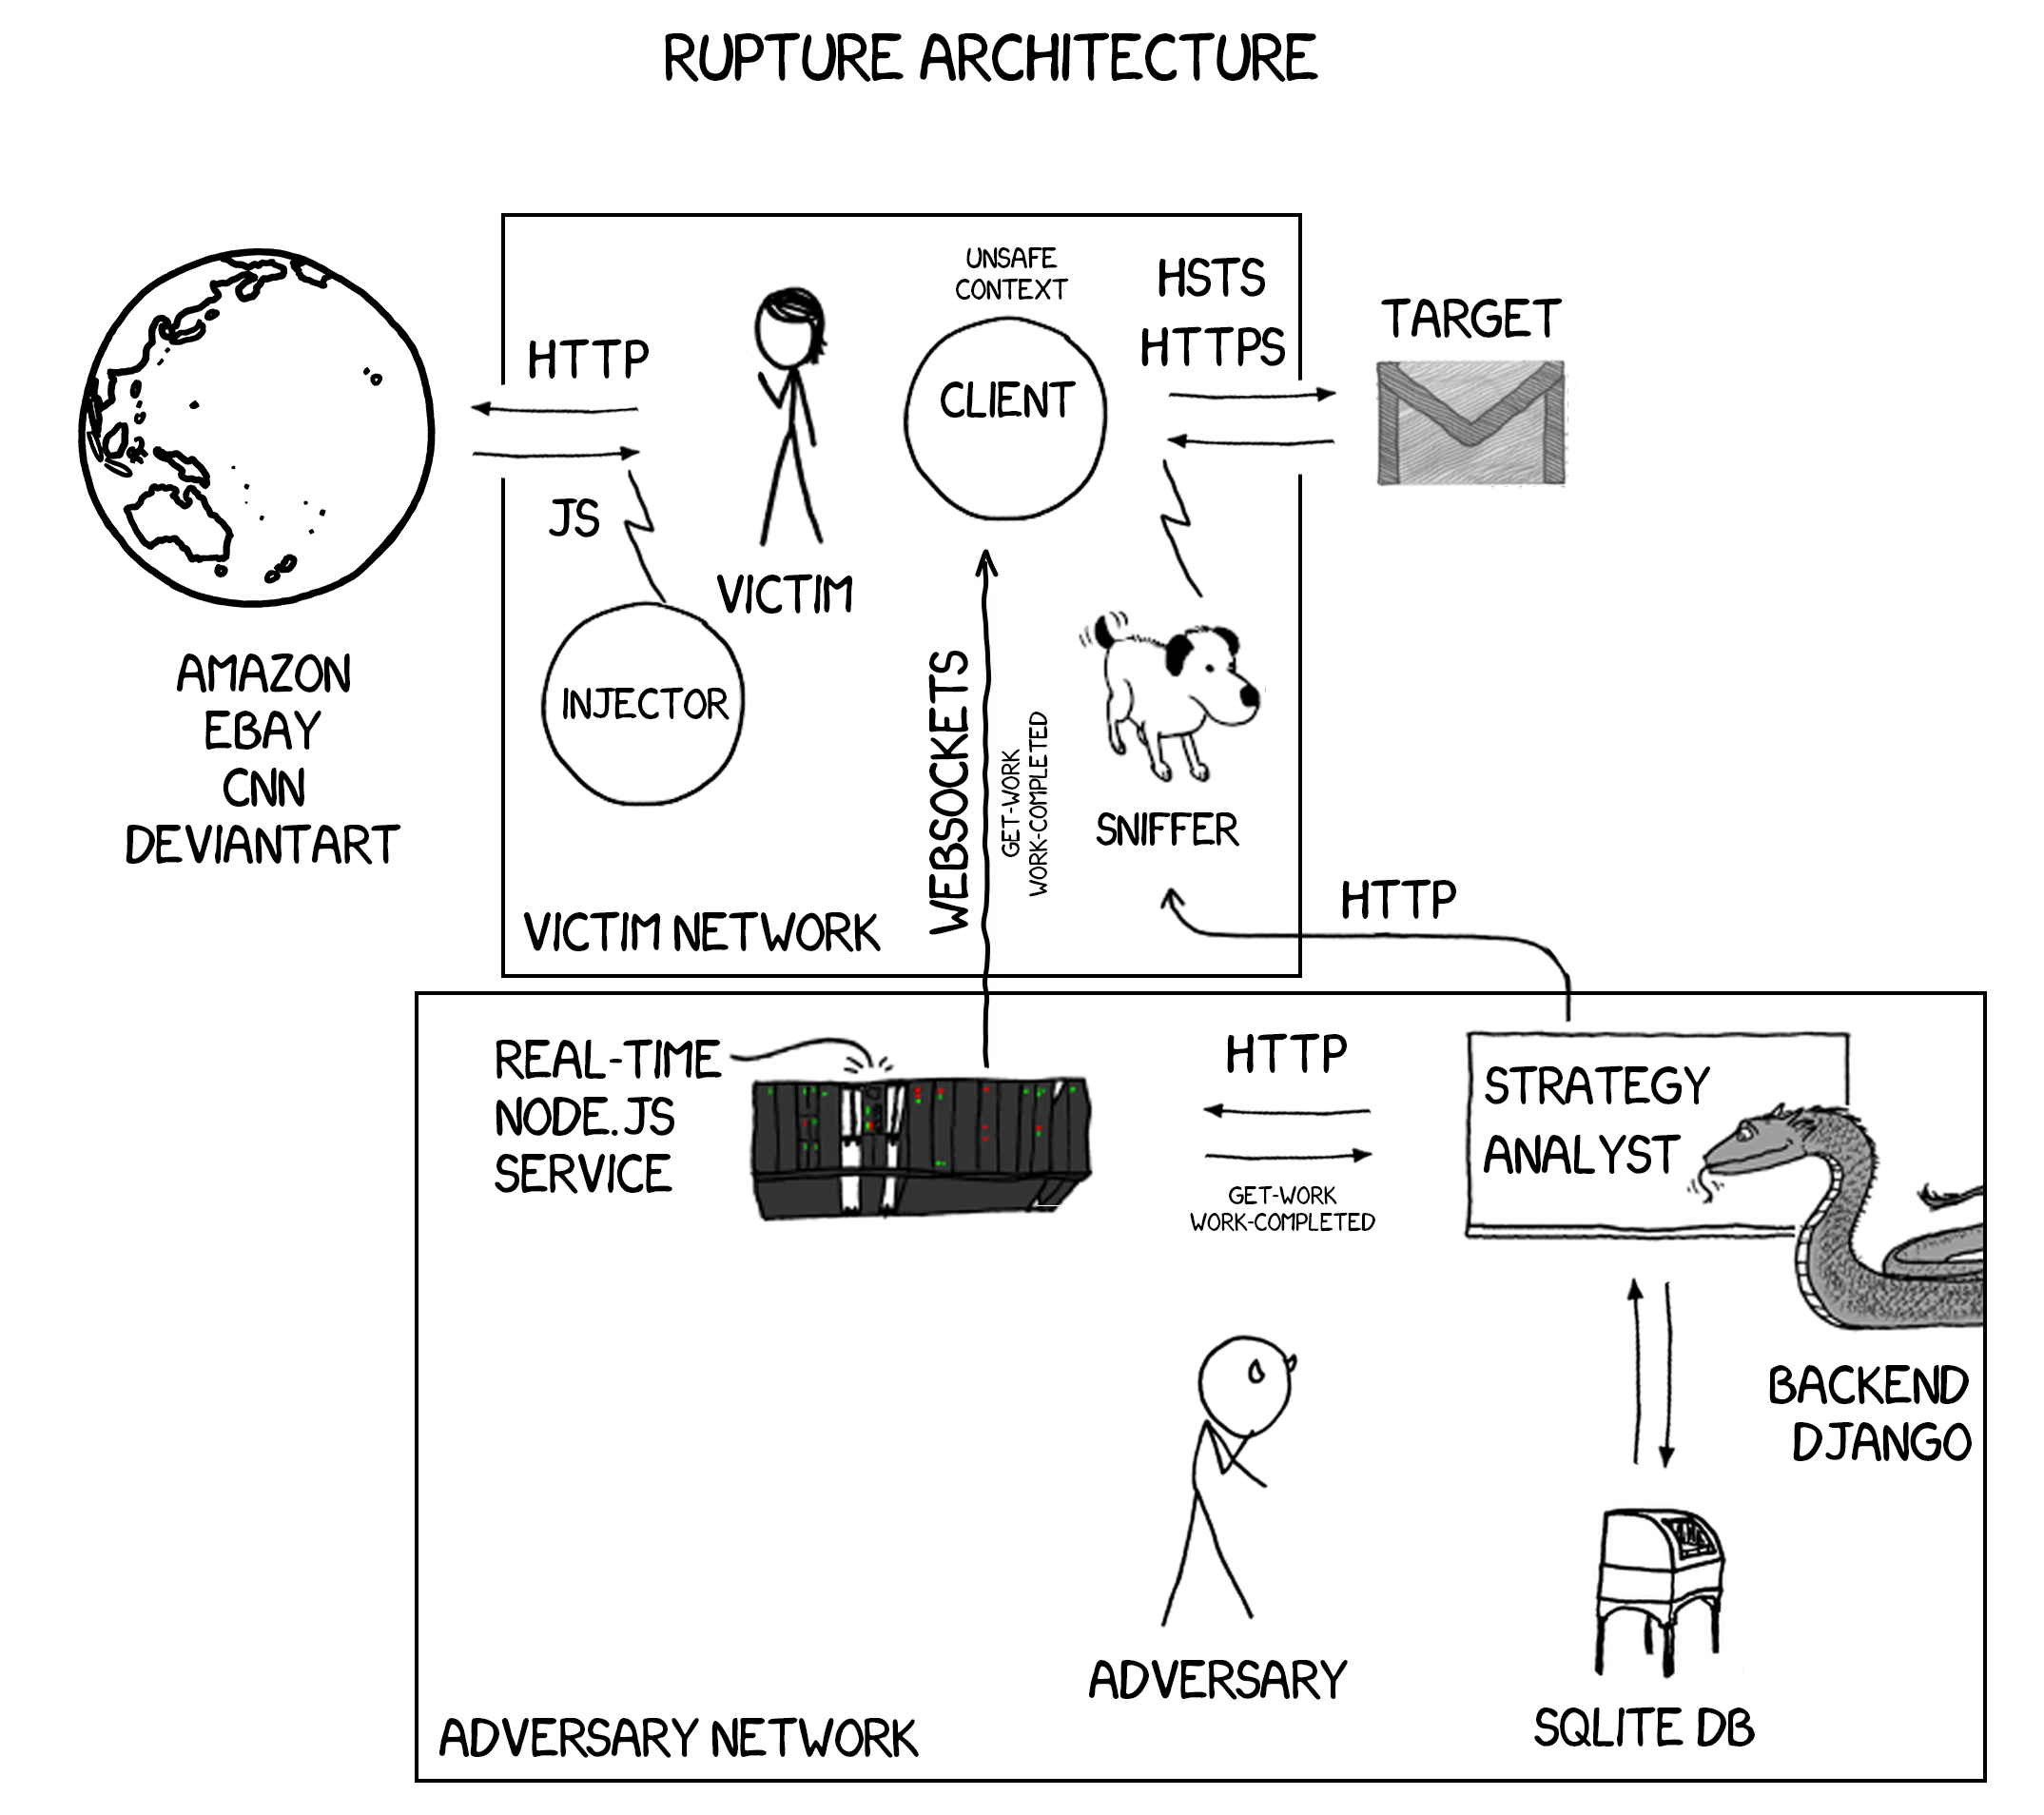
\includegraphics[width=0.48\textwidth]{architecture.png}
      \caption{Rupture Architecture}
   \end{figure}

\section{Practical optimization methods}\label{app:optimization}

\subsection{Block alignment}\label{subsec:blockalign}
Block ciphers are \textit{length monotonic}, but not \textit{strictly length
monotonic}, as described in section \ref{subsec:lenmonotone}. Specifically, the
length of the encrypted text is rounded to a product of $\mu$-bits, where $\mu$
is the block size, using added padding. The same applies for stream ciphers,
whose functionality is similar to block ciphers with block size 1 byte. In this
case, plaintext length difference between two messages does not always result in
length difference between the respective encrypted ciphertext.

It is possible to bypass this problem by using block alignment. Block alignment
techniques have already been explored in the literature \cite{c14}.  This method
demands issuing multiple requests to the reflection oracle while including
artificial noise in the reflection string $r$.  That way, one out of
$\ceil{\mu / |r^i|}$ requests, where $|r^i|$ is the length of one digit of
$r$ in bits, will result in a block distinction between different reflection
strings $r_i$.

\subsection{Reflection computation methods}\label{subsec:reflectionmethods}
Reflection strings $r$ should be polynomially computable, as defined in
\ref{sec:propertycom}. BREACH, defined in \ref{subsec:breachapp}, is
parameterized with an alphabet of ASCII symbols $\mathcal{S}$ for each character of the
secret. A successful attack should distinguish a single character of the
alphabet as the correct one through a series of requests to the reflection
oracle.

The first method of issuing requests is serial. Each request to the oracle
corresponds to a single character of the alphabet. An attack phase is completed
when requests have been issued for the entire alphabet.

In this case, $Q$ is the property "Given a known prefix $p_s$ of secret $s$ and
a symbol $t \in \mathcal{S}$, is $p_s:t$ a prefix of $s$?" and $\exists
s_i \in \mathcal{S}: Q(s_i)$ and $\forall s_j \in \mathcal{S} \setminus \{s_i\}:
\lnot Q(s_j)$. The complexity of the attack is $\mathcal{O}(|\mathcal{S}|)$ and
the round ends by finding a character of the secret.

The second method of attack is divide and conquer. In each phase the alphabet is
divided into two subsets $\mathcal{S}_1$ and $\mathcal{S}_2 = \mathcal{S}
\setminus \mathcal{S}_1$, where $|\mathcal{S}_1| = |\mathcal{S}_2| =
\ceil{|\mathcal{S}| / 2}$. The reflection string for $\mathcal{S}_1$ composes of
$|\mathcal{S}_1|$ substrings divided by an annotation symbol $\beta$. Each
substring consists of the known part of the secret concatenated with a character
in $\mathcal{S}_1$. The reflection string for $\mathcal{S}_2$ is constructed
similarly. Each phase consists of one call to the reflection oracle per subset.

Property $Q$ is defined "Given a known prefix $p_s$ of secret $s$, is $p_s:t$ a
prefix of $s$, where $t \in \mathcal{S}_1$?". As long as the prefix of the
secret is \textit{compression-detectable} by each substring of the reflection,
the end of each phase marks the choice of subset $\mathcal{S}_i$ that contains
the correct alphabet symbol and the same method is applied using chosen
$\mathcal{S}_i$ as the alphabet $\mathcal{S}$. The round is complete when
$|\mathcal{S}| = 1$. Each round reduces the alphabet by half, so the complexity
of the attack with the divide and conquer method  is
$\mathcal{O}(log_2|\mathcal{S}|)$.

\subsection{Request parallelization}\label{subsec:parallel}
The reflection oracle is generally considered as synchronous. However, this is not
always the case, since it may be able to handle multiple parallel requests from
the adversary.

This is the case for the oracle in the practical BREACH application, described
in \ref{subsec:breachapp}. In that case the reflection oracle is an endpoint
offered by a web application and the communication channel between the adversary
and the oracle is the end-to-end browser-server network channel.

Modern web servers are able to handle multiple parallel requests and
browsers can issue a certain amount of parallel requests per domain. This
functionality enables the adversary to issue multiple parallel requests per
symbol in alphabet $\mathcal{S}$ and efficiently reduce the execution time of
the attack.

\subsection{Request soup}
Previous sections demonstrated the need for multiple requests per reflection
string $r_i$. However, it is often the case that communication with the
reflection oracle given consequent analysis of each single request is time
expensive. In this case, it is preferable to issue multiple indistinguishable
requests and treat them as a set for the relative symbol.

This technique is useful in the case of the BREACH attack described in
\ref{subsec:breachapp}. In this case, communication between the browser and the
endpoint that serves as the reflection oracle is encrypted, so the analysis of
the captured packets is time expensive per request set.

A request set consists of requests for a symbol $s_i$ in alphabet $\mathcal{S}$,
so bigger request sets result in less time delay. Length calculation per request
can then be measured as the mean length over the number of requests in the set.

This method can be combined with the methods described in \ref{subsec:parallel}
in order to utilize the parallelization and reduce the time cost of the
necessary multiple requests.

\section{Related work}\label{sec:related}

\subsection{Defenses}

Defense against side-channel compression attacks and especially BREACH have been
proposed in bibliography, including \cite{c3}, \cite{c5} and \cite{c6}.

\subsubsection{Disabling compression}\label{subsec:disablecom}
Compression is the basic assumption for property compressibility. Disabling
compression would break the adaptive reflection game, since it removes
the compression part of the encryption function.

However, this method is not viable, since the performance overhead should it be
applied overrules the benefits of the defense.

\subsubsection{SameSite cookies}\label{subsec:samesite}
SameSite cookies \cite{c10} is a proposed draft for enhancing web security. The
main puprose of this technique is to mitigate cross-site request forgery
attacks, although it also mitigates other kinds of cross-origin leakages.

This policy introduces a new attribute for web cookies that web servers may
opt-in. This attribute states that cookies may only be included in a
"first-party" context, i.e. in same origin requests.

However, the current BREACH application depends on cross-origin requests in
order to call the reflection oracle, as defined in \ref{subsec:breachapp}.
Enabling SameSite cookies would result in the elimination of this reflection
oracle of the Reflection-Security Game and the effective mitigation of the
attack.

\subsubsection{Masking secrets}\label{subsec:masking}
Masking is a method of hiding secrets' properties per request. A mask is a
bitstream equal in size with the secret. The masked text contains the result of
the XOR operation between the secret and the mask concatenated with the mask.
The secret can be obtained by applying XOR between the first and the second
half of the masked text.

A masking function is defined:

\begin{lstlisting}[texcl,mathescape,basicstyle=\small]
def masking($s_i$):
    $l = |s_i|$
    $m_i \xleftarrow{\$} \{0, 1\}^l\\$
    $s_i' = m_i \oplus s$
    return $s_i', m_i$
\end{lstlisting}

Masking can be applied on a rendered secret $s_i$ in the output $m$ of a
rendering function $f$ as:

\begin{lstlisting}[texcl,mathescape,basicstyle=\small]
def apply_masking($m_i, s_i$):
    $s_i', m_i \leftarrow masking(s_i)$
    return $Rep(m, s_i, \beta_1 s_i' \beta_2 m_i \beta_3)$
\end{lstlisting}

where $Rep$ is the string replacement function defined in
\ref{subsec:rendering} and $\{\beta_1, \beta_2, \beta_3\}$ are symbols that do not
appear in $m$ before masking.

Mask removal should be applied on all masked secrets, marked by the annotation
symbols $\beta_1$, $\beta_2$, $\beta_3$, before the reversing of rendering function $f$:

\begin{lstlisting}[texcl,mathescape,basicstyle=\small]
def remove_masking($m', \beta_1, \beta_2, \beta_3$):
    return $Rep(m', \beta_1 s_i' \beta_2 m_i \beta_3, s_i' \oplus m_i)$
\end{lstlisting}

where $Rep$ is the string replacement function and $\{\beta_1, \beta_2,
\beta_3\}$ are the annotation symbols used in \texttt{apply\_masking}.

Mask $m_i$ is chosen uniformly at random, so masked secret $s_i'$ is also
random. This results in $s_i' m_i$ being indistinguishable from $r_1 r_2$ by a
compression function $Com$, where $r_1$, $r_2$ are random nonces chosen
uniformly at random.

Masking renews the secret $s_i'$ each time the reflection oracle is called. That
way, this method secures the secret's content against instances of the attack
that require at least two calls to the reflection oracle.

Masking doubles the size of the secret that is being protected. Furthermore,
$m_i$ and $s_i'$ are random, so the compression performance is poor. Therefore,
masking should be applied with limitation on high value secrets only, in order
to avoid significant performance drop.

Masking is a method used by Facebook \cite{c11} in order to protect CSRF tokens
against BREACH attacks.

\appendices

\section{The compression function assumption}\label{subsec:comfuncassumption}

In BREACH, $Com$ is a variant of LZ77 \cite{c9}. In this compression algorithm,
repetitions of strings are well-compressed. In our ideal model, we examine a
simplified version of LZ77 which we describe in this paragraph.

Our version of LZ77 is not composed with a symbol-compressing algorithm such as
Huffman coding. Therefore, a way is needed to encode literal symbols and
compression symbols. The LZ77 algorithm treats the uncompressed text as a
series of bits. Let the plaintext be $p$ and its length be $n = |p|$. The LZ77
compression function needs to have an alphabet of 2 symbols for representing
literals (the bits $0$ and $1$ of the plaintext) as well as an alphabet of an
additional $n$ symbols for representing compression distances from $1$ to $n$
and lengths from $1$ to $n$ (the same symbol is used to represent a distance
and a length). This makes an alphabet of a total of $n + 2$ symbols which are
represented by bit sequences of exactly $\ceil{lg(n + 2)}$ bits each.

We first describe the decompression algorithm. At the beginning of the
compressed string, the number of characters in the uncompressed plaintext is
encoded in ASCII followed by the "$\$$" ASCII character as a separator. This
allows the decoder to compute how many bits are used to represent each symbol
in the compressed text.

Ordering these bit strings lexicographically, the first two bit strings will
correspond to the literal "$0$" and "$1$" bits of the plaintext. The next bit
strings will correspond to \textit{distance} bit sequences of values $1, 2,
\ldots, n$ respectively.

After the "$\$$" separator, an encoding of the plaintext is given. The encoding
can be decompressed by linearly reading it one character at a time. If a bit
sequence corresponding to a literal is given, this is decoded as the respective
literal bit of the plaintext. If a distance bit sequence of value $a$ is given,
then another distance bit sequence of value $b$ sequence follows.  Then $a$
must be less than or equal to the plaintext characters decoded so far, while
$b$ is arbitrary. This pair of values is decoded as follows. The decompressed
text beginning at a distance of $a$ bits behind the current position decoding
position and of length $b$ bits is taken into account. That text is then the
new decompressed plaintext which is appended to the existing decompressed
plaintext one bit at a time. This procedure can cause self-overlapping texts.
In the end, the decoded text must be $n$ bits long, otherwise the compression
is invalid.

\begin{lstlisting}[texcl,mathescape,basicstyle=\small]
def $\text{LZ77}^{-1}(c)$:
    parts = c.split("$\$$")
    plaintextLength = parse_int(parts[0])
    bitsPerSymbol = $\ceil{lg(\text{plaintextLength}) + 2}$
    enc = strToBinArray("".join(parts[1:]))

    plaintext = ''
    for i in range(0, len(enc), bits):
        symbol = binaryToInt(enc[i:bits])
        if symbol = 0:
            plaintext += '0'
        else if symbol = 1:
            plaintext += '1'
        else:
            d = symbol - 1
            i += bits
            length = int(enc[i:bits])
            if d > len(plaintext):
                return $\bot$
            while length:
                plaintext += plaintext[-d]
                length -= 1
    if len(plaintext) != plaintextLength:
        return $\bot$
    else:
        return plaintext
\end{lstlisting}

Where negative and range array indexing and the $range$ function is as in
Python.

Our LZ77 compressor can then be described simply: It chooses the shortest in
bits compressed text, which, when decoded using the above algorithm yields the
desired plaintext.

% TODO: Prove that it is a compression function for some $\mathcal{M}$

\section{The BREACH model}\label{sec:breachmodel}
We now turn our attention to the BREACH attack specifically, which utilizes
the properties explored above, and we describe that BREACH is a specific
instance of the general attack.

In the BREACH model, we deal with a specific function $f$, property $Q$,
compression function $Com$, length-leaking $Enc$, and secret distribution
$\mathcal{M}$.

In the next paragraphs, we describe a simplified model of the attack that
lends itself to the formal model, while abstracting away the complex
practical details of the attack pertaining to the networking and particularities
of the implementation that are of little significance to the cryptographic
formalisms presented here.

\subsection{The rendering context assumption}\label{subsec:rendering}

In the modern web, function $f$ represents a specific attack target, which
constitutes the renderer of a web page, given a specific secret, reflection,
and noise. Typically, $f$ will concatenate instances of the secret, the
reflection, and the noise, between some context strings which constitute the
static portions of the site.

In the case of BREACH, it is typically assumed that $f$ outputs a concatenation
of various instances of $s$, $r$, and $v$ with arbitrary repetitions, in
addition to concatenating with some constant context whose position is
independent of the values of $s, r, v$. The number of repetitions of $s, r, v$
are also independent of the values of $s, r, v$.

Formally, assume that the symbols $\{\beta_1, \beta_2, \beta_3\}$ do not appear
in the alphabet of the secret.

Our assumptions for $f$ can be stated as follows. Let
\begin{equation*}
\begin{split}
\exists \mu \in \{0, 1, \beta_1, \beta_2, \beta_3\}^*\\
\exists u_1, v_1, u_2, v_2, u_3, v_3 \in \{0, 1, \beta_1, \beta_2, \beta_3\}^*\\
\mu = u_1 \beta_1 v_1 \land\\
\mu = u_2 \beta_2 v_2 \land\\
\mu = u_3 \beta_3 v_3 \land\\
\forall s, r, v \in \{0, 1\}^*\\
f(s, r, v) = Rep(Rep(Rep(\mu, \beta_1, s), \beta_2, r), \beta_3, v)
\end{split}
\end{equation*}

Where $Rep$ is the string replacement function:
\begin{align*}
Rep(\epsilon, \alpha, \beta) &\defeq \epsilon\\
Rep(\alpha:xs, \alpha, \beta) &\defeq \beta:Rep(xs, \alpha, \beta)\\
Rep(x:xs, \alpha, \beta) &\defeq x:Rep(xs, \alpha, \beta)
\end{align*}

Where $:$ denotes the concatenation of a symbol with a string.

We call $f$ functions that exhibit such behavior \textit{concatenative}.

\subsection{The full-text predicate assumption}\label{subsec:fulltextassumption}

The BREACH attack is a specific instance of reflection-based attacks in which
the $Q$ property pertains to a prefix of the secret. It asks "Does the secret
begin with such text?"

We require $X$ to be of compressible length,
i.e. the following equation must be satisfied:
\begin{equation*}
    |X| > \ceil{lg(f(X, X, \epsilon) + 2)}
\end{equation*}

In practical terms, this requires the secret that needs to be stolen to be at
least 3 bytes so that it is better compressed rather than represented as a
literal.

\subsection{Prefixes are
compression-detectable}\label{subsec:breachprefix}

Let $startswith(v, s)$ be the $k$-length prefix checking predicate on a
$\lambda$-bit secret $s$:
\begin{equation*}
    startswith(v, s) \defeq \exists w: s = v w
\end{equation*}

Let $f$ be a concatenative rendering function and let $Com = LZ77$. Then:
\begin{align*}
\Pr[startswith(v, \cdot) \textrm{ compression-detectable under } f, Com] =\\ \text{non-negl}(\lambda - k)
\end{align*}

Where the probability randomness is taken uniformly over all $k$-bit prefixes $v \in \{0, 1\}^k$.

Due to the complexity of the $LZ77$ algorithm, we do not provide a proof of this result. However, the
result has been experimentally verified against various end-points by our open-source Rupture implementation.
This result is also supported by the feasibility of BREACH and CRIME.

\begin{thebibliography}{13}

\bibitem{c1} J. Rizzo and T. Duong, "The CRIME attack", Ekoparty, 2012.

\bibitem{c2} Be'ery, T. and A. Shulman, "A Perfect CRIME? Only TIME Will Tell",
Black Hat Europe 2013, 2013.

\bibitem{c3} Y. Gluck, N. Harris and A. Prado, "BREACH: Reviving the CRIME attack",
Black Hat USA, 2013.

\bibitem{c4} John Kelsey, "Compression and information leakage of plaintext", 2002.

\bibitem{c5} J. Kelley and R. Tamassia, "Secure Compression: Theory \& Practice",
2014.

\bibitem{c6} J. Alawatugoda, D. Stebila and C. Boyd, "Protecting encrypted
cookies from compression side-channel attacks", 2014.

\bibitem{c7} D. Karakostas and D. Zindros, "Practical New Developments on
BREACH", Black Hat Asia, 2016.

\bibitem{c8} NIST, "Announcing the ADVANCED ENCRYPTION STANDARD (AES)", 2001.

\bibitem{c9} J. Ziv and A. Lempel, "A universal algorithm for sequential data
compression", Information Theory, IEEE Transactions, vol. 23, 1977.

\bibitem{c10} M. West, "First-Party-Only Cookies", RFC Internet-Draft, 2015.

\bibitem{c11} [online] URL:
\url{https://www.facebook.com/notes/protect-the-graph/preventing-a-breach-attack/1455331811373632}
[cited November 2016]

\bibitem{c12} P. Deutsch, "DEFLATE Compressed Data Format Specification version
1.3", RFC 1951, 1996.

\bibitem{c13} [online] URL: \url{https://ruptureit.com} [cited November 2016]

\bibitem{c14} B. Moller, T. Duong, K. Kotowicz, This POODLE Bites: Exploiting the SSL 3.0 Fallback, September 2014.

\bibitem{c15} T. Dierks, E. Rescorla, The Transport Layer Security (TLS)
Protocol Version 1.2, August 2008.

\bibitem{c16} [online] URL:
\url{https://www.owasp.org/index.php/Cross-Site_Request_Forgery_(CSRF)} [cited
November 2016]

\bibitem{c17} R. Fisher, F. Yates: Statistical tables for biological,
agricultural and medical research, 1938

\bibitem{c18} M. S. Mayzner, M. E. Tresselt, Tables of Single-letter and Digram
Frequency Counts for Various Word-length and Letter-position Combinations, 1965

\bibitem{c19} [online] URL:
\url{https://w3techs.com/technologies/details/ce-gzipcompression/all/all} [cited
November 2016]

\end{thebibliography}

\end{document}
